\chapter{Lecture five: Usage}

\section{Application Domain Analysis}
Application-domain analysis focuses on a question: How will the target system be used? The purpose is to define requirements for the system's functions and interfaces.

\subsection{Result}
A complete list of the system's overall usage requirements. This includes actors and use cases, user interfaces and functions. 

\subsection{Key concepts}
\textbf{Application domain:} The organisation that administrates, monitors, or controls a problem domain. 

\subsubsection{New concepts}
New concepts in the application domain analysis includes:
\begin{itemize}
    \item Actors (users and other systems)
    \item Use cases
    \item Functions
    \item Interfaces
\end{itemize}

\subsection{Using the model of the problem domain}
Stage's infamous penis-model-drawing is included here.
\textbf{Model:} A description of classes, objects, structures, and behaviour in a problem domain. Provides an updated representation of the state in the problem domain. 

In analysis, we describe the problem domain by an object-oriented model. We also describe how the model is used in the application by the actors.

\subsection{Activities}
This is the finding of usage, functions, and interfaces. Defining requirements is an iterative activity alternating between usage, functions and interfaces. These three will be discussed in chapters 6-8.

\begin{table}[]
\centering
\begin{tabular}{lll}
\hline
\multicolumn{1}{|l}{\textit{\textbf{Activity}}} & \textit{\textbf{Content}} & \multicolumn{1}{l|}{\textit{\textbf{Concepts}}} \\ \hline
Usage & \begin{tabular}[c]{@{}l@{}}How does the system interact \\ with people and \\ systems in the context?\end{tabular} & Use case and actor \\
Functions & \begin{tabular}[c]{@{}l@{}}What are the sytem's\\ information processing \\ capabilities?\end{tabular} & Function \\
Interfaces & \begin{tabular}[c]{@{}l@{}}What are the target system's \\ interface requirements\end{tabular} & \begin{tabular}[c]{@{}l@{}}Interface, user interface,\\ and system interface\end{tabular} \\ \hline
\end{tabular}
\end{table}

\subsection{Stable versus transient properties}
The different properties in the system has different levels of stability. When the model is changed, all the functions and interfaces must change also. However, the functions can be changed, without changing the model. Interfaces can also be changed, without changing the functions or the model. The model is therefore more stable. In practice, the system model changes more rarely than the function or interface requirements.

\begin{figure}[H]
    \centering
    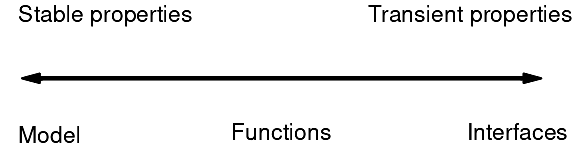
\includegraphics[width=.6\textwidth]{figures/properties.png}
\end{figure}

\subsubsection{Classical vs modern bank}
The model is the same. The basic functions are the some, withdraw and deposit, but new ones are added, e.g. MobilePay. Interfaces are however completely changed.
\begin{table}[h]
\centering
\begin{tabular}{|l|l|l|}
\hline
 & Classical bank & Modern bank \\ \hline
Model & Identical & Identical \\ \hline
Function & Withdraw and deposit & Also with/deposit, however also transactions \\ \hline
User interface & Different & Different \\ \hline
\end{tabular}
\end{table}

\subsection{Summary}
\begin{figure}[H]
    \centering
    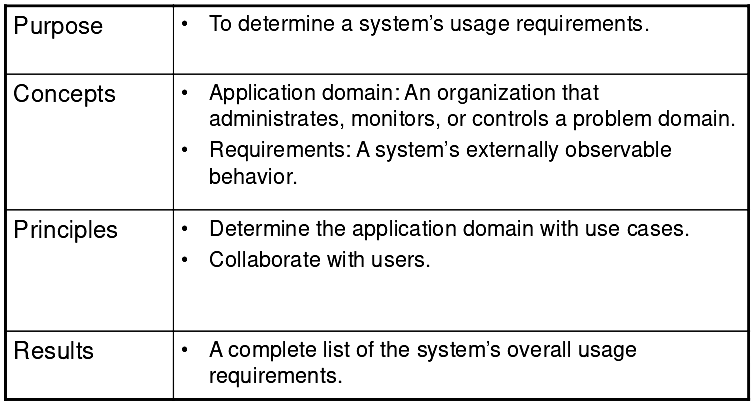
\includegraphics[width=.6\textwidth]{figures/apdomainsummary.png}
\end{figure}

\section{Usage}
\subsection{Results}
Descriptions of all \textbf{use cases}, \textbf{actors}, and an \textbf{actor table}.
\begin{figure}[H]
    \centering
    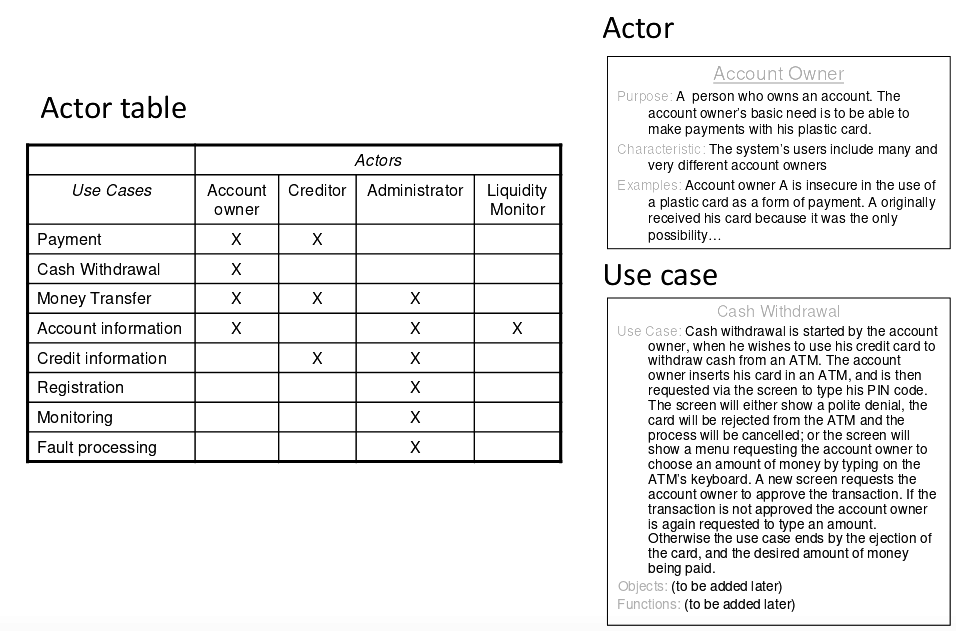
\includegraphics[width=\textwidth]{figures/usageresults.png}
\end{figure}

\subsection{Start out from work tasks}
What tasks exist in the application domain? How is the division of labour? How are the different tasks delimited?

\noindent Describe the tasks:

\begin{itemize}
    \item Name and content
    \item Purpose
    \item How is it assigned?
    \item Who performs it?
    \item Relationship to other tasks
    \item Result
\end{itemize}

For example, an administration system's work tasks:

\begin{itemize}
    \item Establish new conference
    \item Detailed planning of conference
    \item Administration of participants
    \item Registration of person
    \item Administration of articles
    \item Information to the committees
    \item Information to participants, authors, and reviewers
\end{itemize}

\subsection{Key concepts}
\subsubsection{Actor}
Identify actors:
\begin{itemize}
    \item Determine the distribution of roles of the work tasks related to the system
    \item Consider human actors
    \item Consider other systems as actors
\end{itemize}

\noindent Lastly, describe these actors in terms of \textbf{purpose, characteristics, and examples}. E.g. an account owner in a bank could be described as the following:

\begin{itemize}
    \item[] \textbf{Purpose:} A person who owns an account. The account owner's basic need is to be able to make payments with his plastic card.
    \item[] \textbf{Characteristic:} The system's users include many and very different account owners.
    \item[] \textbf{Example A:} Account owner A is insecure in the use of a plastic card as a form of payment. A originally received his card because it was the only possibility for getting an ID card for his checks. A only withdraws money from the ATM in emergency situations.
    \item[] \textbf{Example B:} Account owner B is technologically curious and uses the system often, optimally, and to the limit of its abilities. B has never had major problems in understanding the possibilities of the system, and B also examines the possibilities that are not obviously available.
\end{itemize}


\subsubsection{Use cases}
Identify use cases where the system is used to carry out part of a work task. Describe use cases; as text or as a state-chart diagram, or an actor-table as seen on page 123.


\noindent A \textbf{use case} based on cash withdrawal could be written like the following:

\begin{itemize}
    \item[] \textbf{Use case:} Cash withdrawal is started by the account owner, when he wishes to use his credit card to withdraw cash from an ATM. The account owner inserts his card in an ATM, and is the requested via the screen to type his PIN code. The screen will either show a polite decline, the card will be rejected from the ATM and the process will be cancelled, or the screen will show a menu requesting the account owner to choose an amount of money by typing on the ATM's keyboard. A new screen requests the account owner to approve the transaction. If the transaction is not approved the account owner is again requested to type an amount. Otherwise the use case ends by the ejection of the card, and the desired amount of money being paid.
    \item[] \textbf{Objects:} \textit{to be added later}
    \item[] \textbf{Functions:} \textit{to be added later}
\end{itemize}

It could also be drawn using behavioural patterns, like the following figure shows:

\begin{figure}[H]
    \centering
    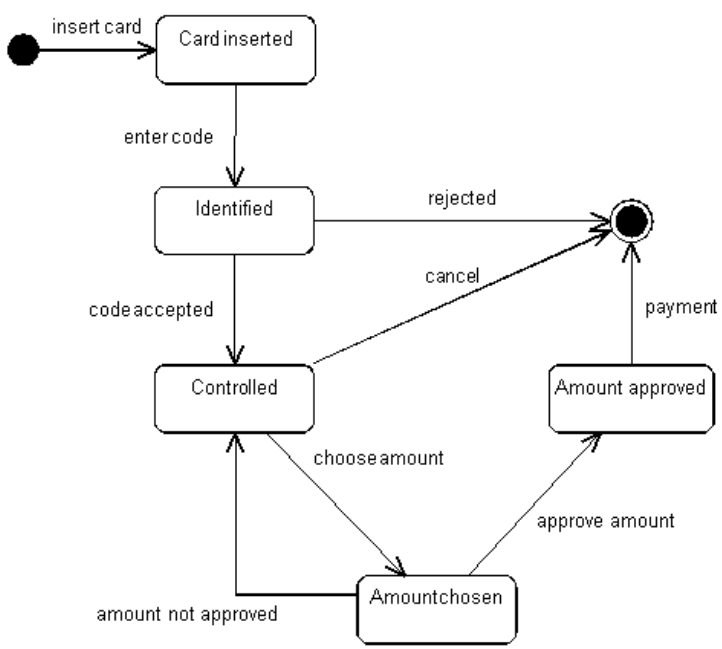
\includegraphics[width=.7\textwidth]{figures/usecasechart.png}
\end{figure}

Note that state-chart diagrams er easy and concise to discuss with peers, but users will only understand a written description of the use case.

\subsection{Activities}
Starting from a a system definition, find actors and use-cases, then both evaluate systematically and explore patterns, which lastly lead to use cases and actors.

\subsection{Evaluate systematically}
The aim is not to get a ton of details, it's to get an idea of the users and what they're doing. Do a systematic review:

\begin{itemize}
    \item Use cases should be simple and constitute a coherent whole. 
    \item The description of actors and use cases should provide understanding and overview. 
    \item Use cases should be described in enough detail to enable identification of functions and interface elements.
\end{itemize}

E.g., what could be functions and interface elements for cash-withdrawal? Also experiment with prototypes, a use case is best evaluated through planned prototype experiments.

\subsection{Summary}
\begin{figure}[H]
    \centering
    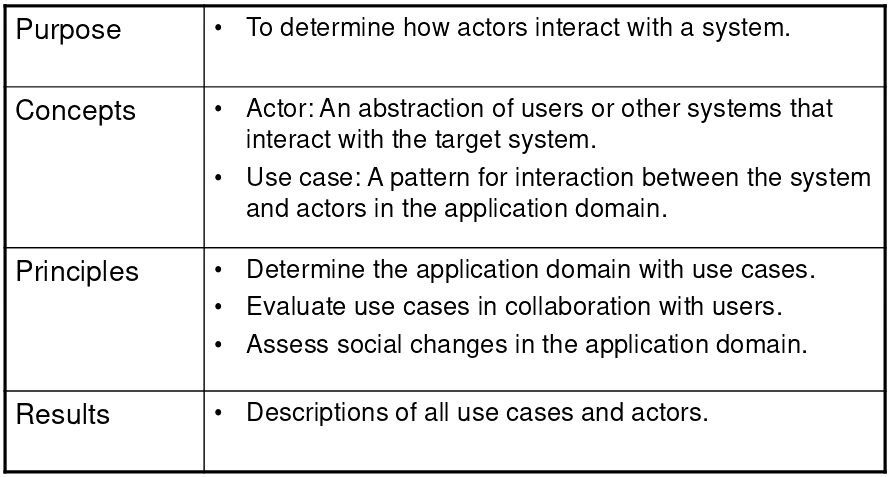
\includegraphics[width=.7\textwidth]{figures/usagesummary.png}
\end{figure}

\section{Example with a streaming service}
Recall previous class diagrams, behavioural patterns, and statechart diagrams, as seen in section \ref{behaviour:streamingservice}. An actor table for the streaming service follows:

\textit{missing from slides and therefore also from notes}

\section{Explore patterns}
\subsection{Procedural pattern}
\begin{figure}[H]
    \centering
    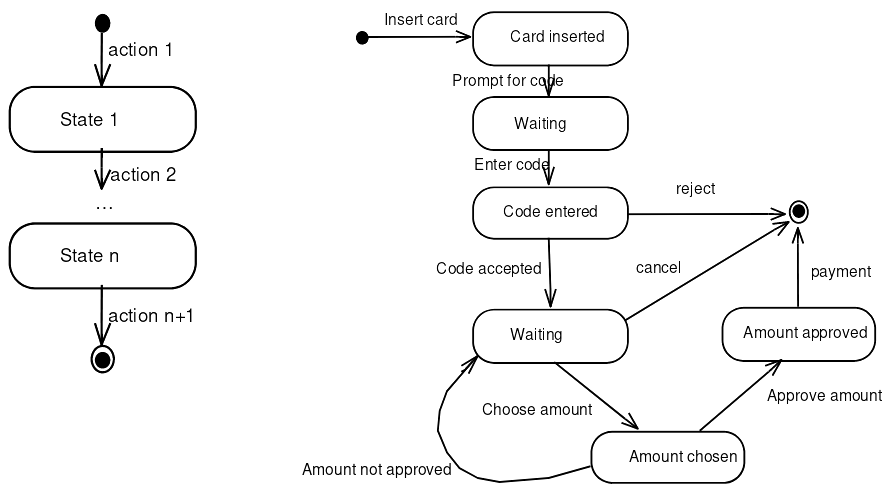
\includegraphics[width=.8\textwidth]{figures/proceduralpattern.png}
\end{figure}

Some cases dictate that certain rules are observed. In cash withdrawal for example, the actor's access rights must be established first, and there must be an extra confirmation of the withdrawal amount. This allows little variation in the actual dialogue. The use case must follow a strict procedure.

The procedural use-case pattern is the general solution to ensuring that many rules are observed. As the figure shows, the patterns basic structure is a sequence with minor variations in terms of selections or iterations. The selections and iterations can be described as nested inside the upper level states.

\subsection{Material pattern}
\begin{figure}[H]
    \centering
    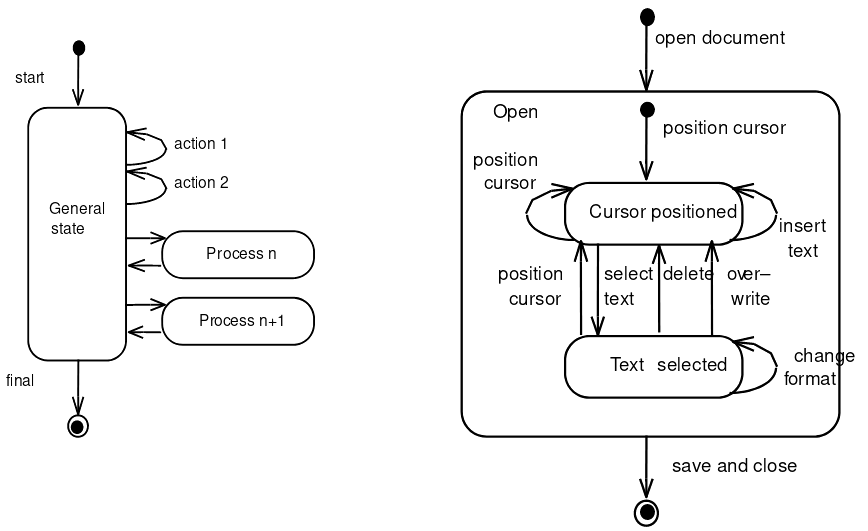
\includegraphics[width=.7\textwidth]{figures/materialpattern.png}
\end{figure}

Consider a text-editing processor. The general use case might look like what's shown in the figure; it is characterised by very little sequence and the actor can do almost anything in any order. The only restriction comes from the two modes; "cursor positioned" and "text selected", which the actor must be in to perform certain actions.

The material use case is good for situations in which there are no business-rules governing the usage. The pattern is a use-case with few general states, in which most actions can be performed. We call this the "material" use case as it resembles an artisan's material process; any tool may be used in any order.

\section{Appreciate the difference; actors and classes}
\begin{figure}[H]
    \centering
    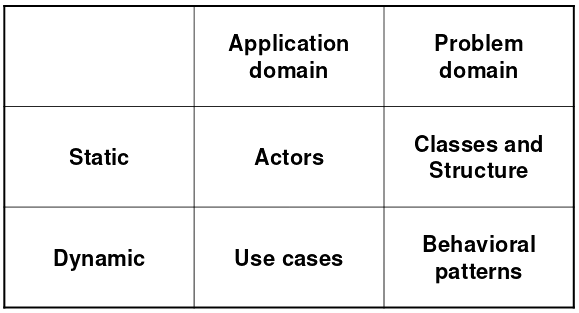
\includegraphics[width=.5\textwidth]{figures/actorvsclasses.png}
\end{figure}

\section{Principles}
\subsection{Determine the application domain with use cases}
Use cases help to focus your analysis on relevant parts of the application domain and provide descriptions at a relevant and homogeneous abstraction level. The use-case activity is an important step toward identifying requirements for the system's functions and interfaces.

\subsection{Evaluate use cases in collaboration with users}
Experiments with prototypes are well suited to use-case evaluation and can provide inspiration for new use cases.

\subsection{Assess social changes in the application domain}
Developing a new system is an opportunity to critically rethink the work organisation in the application domain. The goal is to avoid work-related problems and unnecessary human adjustments.